Welcome to the second instalment of AiRM, this time taking a look at
\textbf{cellular automata}.

We have some exciting articles lined up for the future, potentially
including but not limited to Chaos Theory, Trans-finite Set Theory, Game
Theory and more - so, watch this space!

To understand what a cellular automaton is, I think it is helpful to
understand the motivation behind the concept's creation in the 1940s,
leading up to a book which essentially founded the field: \emph{The
Theory of Self-Reproducing Automata} by \textbf{John von Neumann}.

In this case, it is also necessary to have a word on John von Neumann,
since he was an exceptional man and potentially merits the term genius
in all the ways he contributed to mathematics. In fact, his remarkable
intelligence was noticeable from a young age, when at just 6 years old,
he was able to proficiently converse in Ancient Greek and became quickly
famous in his school for being able to multiply and divide 8-digit
numbers in his head in under 10 seconds.

By 15, he was under the tutelage of Gabor Szego (a mathematician famous
for his contributions to calculus and linear algebra), had a great
understanding of most founding fields of higher mathematics and at age
19, he published his first mathematical papers. \emph{Hans Bethe}, Nobel
Prize winning physicist, was a long-time friend of von Neumann's. When
Bethe observed von Neumann talking with his baby daughter Marina, he
noticed that ``John'' could very easily lower himself so that they were
able to talk as equals and then wondered if von Neumann used just the
same approach when talking to his physicist friends.

By the 1940s, von Neumann had become interested in self-replication. He
wanted to comprehend on an abstract level how a dynamic system or
mechanistic object like life on earth could go about creating copies of
itself in an efficient way and one that could allow for variation (a
property referred to as \emph{evolvability}) -- he came to the
conclusion that it ultimately relied upon:

\begin{itemize}
\item
  The propagation of information in systems.
\item
  The culmination of well-defined local rules into complex global
  behaviour.
\item
  The information structure (or ``tape'' as he called it) being an
  active part of the construction process.
\end{itemize}

Consider that these observations were made prior to the discovery of the
structure of DNA. von Neumann had, in a heuristic sense, understood what
it had to look like.

To define a cellular automaton, consider an \(n\)-dimensional space (a
plane, say) divided into discrete unit-squares, where each square is a
\emph{cell} which can be in one of a defined number of states. Then, we
wish to propagate each cell to a new state with the use of a
\emph{ruleset}, where we look at a \emph{neighbourhood} of defined
nearby or local cells for a given cell and based on their states, we
assign that cell its next state. The ruleset itself is an ordered list
of sets-of-length 2 containing every possible configuration of the
neighbourhood and a state assigned to that.

This sounds quite abstract, so to illustrate, we can take a look at one
of the elementary automata, discovered in the 1980s by Stephen Wolfram.

\begin{figure}[htbp]
\centering

\includegraphics{image_0.png}
\caption{}
\end{figure}

This particular automaton is 1 dimensional, has 2 states and is named
\textbf{\emph{Rule 110}}, as you can see. Since Rule 110's neighbourhood
for a given cell consists of the cell itself \& the two cells directly
adjacent to it (thus, having size 3) and since there are 2 states, the
number of possible configurations of the neighbourhood is \(2^3\),
represented by the 8 boxes at the top just below the name. The row of
three in a given box denotes a particular neighbourhood configuration
(for example, the far right box is where the neighbourhood cells are
only in State 0) and the cell in the middle column below it shows the
defined outcome for that situation, which can be notated as a number in
general from \(1,2,…,n\) where the number of states is
\(n∈\mathbb{N},n>0\).

You should notice that the boxes are arranged in a systematic order,
gradually moving cell by cell down to the situation where all cells are
in State 0. Thus, by numbering each situation with its state number like
in the image, we can think of each situation as a digit in a base-\(n\)
number unique to that ruleset. For this automaton, this number is
``01101110'' which in base-10 is \emph{110} -- these numbers are called
\textbf{\emph{Wolfram numbers}} after the aforementioned Wolfram began
to catalogue thousands of cellular automata to understand them
experimentally using this notation.

The image below the boxes starts with a one dimensional \emph{lattice}
and a single State 1 cell and every row below it shows an iteration of
the system by using the ruleset shown above. In fact, Rule 110 holds
particular meaning as a cellular automaton, since it was proven to be
computational universal, i.e.~it transfers information between cells in
such a way that in rather specific situations, found by the
mathematician Matthew Cook, one can encode numbers in binary form into
it and perform computations or run programs on these numbers. While the
proof itself and perhaps even the proper statement of the theorem is
quite complicated and beyond the scope of \emph{AiRM}, we can show you
illustrations of information transfer within Rule 110. For example,
there are numerous kinds of spaceships, configurations of cells that
move as a single unit:

\begin{figure}[htbp]
\centering
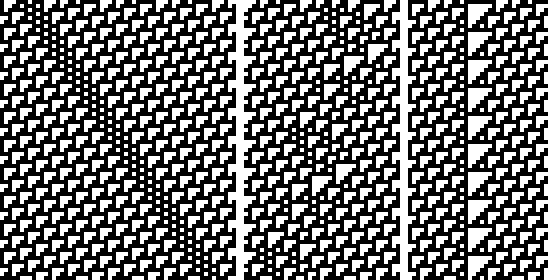
\includegraphics{image_1.png}
\caption{}
\end{figure}

And here they collide:

\begin{figure}[htbp]
\centering
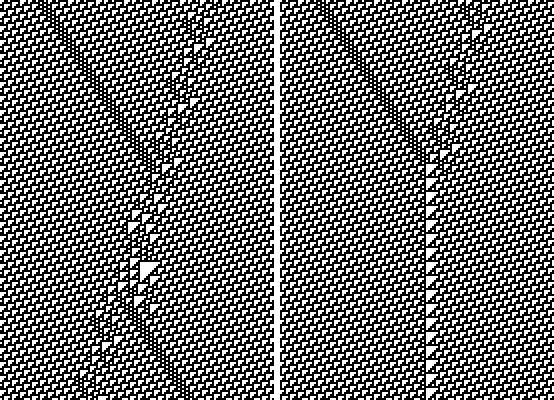
\includegraphics{image_2.png}
\caption{}
\end{figure}

Unfortunately, the proof mentioned was withheld for around a decade
since Wolfram wanted it to be first mentioned in his nascent tome,
\emph{A New Kind of Science}, forcing Cook to not publish one of his
most proud achievements as an employee of \emph{Wolfram Research}.
Eventually, when Cook published early, Wolfram attempted to sue him for
breaking a non-disclosure agreement\ldots{} We at AiRM believe it is
always bad when the spread of intellectual work is inhibited and this
should never happen again.

However, we must return to John von Neumann and his design for a
self-replicating machine: while Rule 110 is only 1 dimensional with 2
states, von Neumann's original automaton had a grand 29 states, was 2
dimensional \& used a neighbourhood which looked at a cell and its four
adjacent cells. As you can imagine, the ruleset would be massive and is
too long to explain here (it required its own book, you see) but we can
give an outline. There was the null or ground State 0 as per usual, a
group of 8 \emph{transmission} states which could act as wires to
transmit binary signals, a group of 4 \emph{confluent} states which
could act as junctions for these wires to give information to \& finally
16 \emph{transition} states which could be built by confluent cells
given the right signals from transmission cells.

The result was an incredible piece of engineering (one which many have
tried fairly unsuccessfully to make simpler): a \emph{universal
constructor}, which, if added to any arrangement of cells in von
Neumann's automaton, would be able to reproduce that arrangement
countless numbers of times. The image below, which I have yet to fully
understand, is taken from WikiCommons based on the work of a
mathematician who actually implemented von Neumann's machine.
Considering the fact that von Neumann made this without the existence of
proper computers that could run simulations of cellular automata, this
is undoubtedly impressive.

\begin{figure}[htbp]
\centering
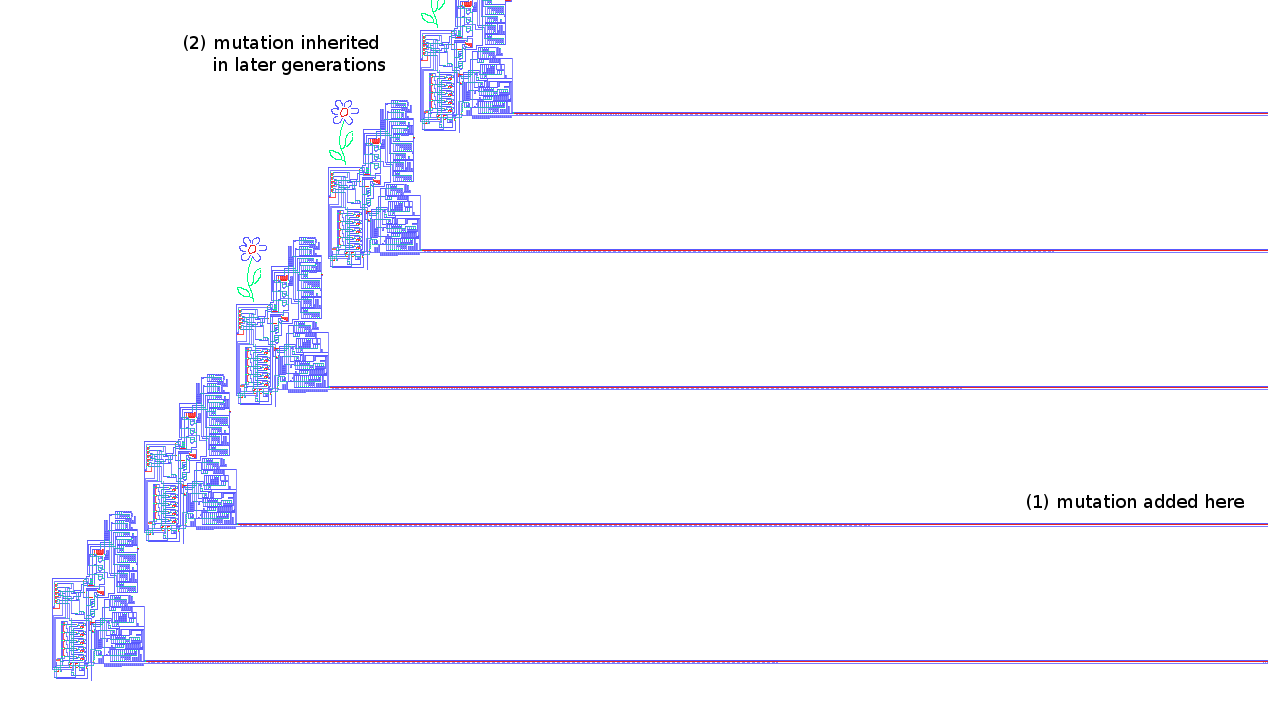
\includegraphics{image_3.png}
\caption{}
\end{figure}

Many mathematicians have considered this work quite astounding due to
the existence of \emph{garden of Eden patterns}, which are a set of
cells with specific states which cannot be formed through iteration of a
previous set, though obviously can act as a starting ``position''. He
apparently accounted for this and since then a much greater
understanding of gardens of Eden has come about due to a theorem proved
by the mathematicians Edward Moore \& John Myhill which states that such
patterns exist for a given cellular automaton if and only if in the
automaton it is possible to construct pairs of structures which after an
iteration ``evolve'' into the same structure.

However, due to the relative obscurity of the work and the fact that his
book was put in the shadow by his many other great works, von Neumann's
universal constructor and indeed the whole idea of cellular automata was
forgotten for around 30 years until a British mathematician,
\textbf{\emph{John Horton Conway}}, created a much simpler 2-state,
2-dimensional automaton whose neighbourhood is the 3x3 block of cells
around \& containing a given cell and which exhibited surprising
complexity. This automaton was called Conway's \emph{Game of Life} and
its rules were the following:

\begin{itemize}
\item
  A State-1 (alive) cell with fewer than 2 State-1 cells in its
  neighbourhood becomes State-0 (dies).
\item
  A State-1 cell with 2 or 3 State-1 cells in its neighbourhood stays at
  State-1.
\item
  A State-1 cell with more than 3 State-1 \emph{neighbours} becomes
  State-0.
\item
  A State-0 cell with exactly 3 State-1 neighbours becomes State-1.
\end{itemize}

With just these four rules come the surprising results that the
automaton is firstly also capable of universal construction, despite
being so much simpler than von Neumann's automaton, that it is capable
of universal computation, like Rule 110 (or just a normal computer) and
finally that for a given starting set of states, the problem of
determining whether the system will eventually evolve to a ``static''
situation (where no further changes happen to the states of any cell in
future iterations of the system) is \emph{generally undecidable},
i.e.~there is no algorithm that solve this problem for all situations.
As Conway said himself ``My life game wasn't designed. I just sort of
thought that if you couldn't predict what it did, then probably that was
because it was capable of doing anything.''

There are many complicated structures, such as analogues of the
previously mentioned spaceships, in the Game of Life. For example, here
is the famous glider:

\begin{figure}[htbp]
\centering
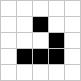
\includegraphics{image_4.png}
\caption{}
\end{figure}

This object will move down diagonally right -- I suggest you take out a
piece of square paper and check with the rules I mentioned \ldots{} or
you could look it up and simply watch one of the many GIFs on
\emph{LifeWiki}, the wiki made by enthusiasts of the automaton which
catalogues thousands of structures made by people and their amazing
properties.

\begin{figure}[htbp]
\centering
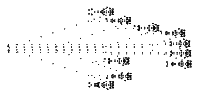
\includegraphics{image_5.png}
\caption{}
\end{figure}

Even more amazing, people have made spaceships which release objects
that release gliders (as in, they make \emph{glider guns})* *
themselves!

Finally, we should consider the work of \textbf{Christopher Langton}, a
somewhat famous mathematician and computer scientist, who founded the
field of \emph{Artificial Life} \& made significant contributions to the
field of cellular automata (for example, creating the Turing-complete
\emph{Langton's Ant}). He described an automaton \emph{invariant} which
he named his \emph{lambda parameter}. One calculates this simply by
taking the ratio \(r\) of the number of configurations of the
neighbourhood that lead to a live or nonzero state to the number of
possible configurations of the neighbourhood and, while simple to
calculate, it brings many revelations.

What Langton observed was that for values of \(λ\) near 0, a randomly
chosen automaton would often be ``ordered'' -- so they would either die
out very quickly or they settle into predictable patterns, and for
values near 1, the automaton would generally display highly chaotic
behaviour. He finally observed that the majority of the complex
automata, which would show groups of cells acting as discrete structures
\& interacting with each other, would often have a \(λ\) value close to
0.5, the boundary which he referred to as the ``edge of chaos''.

Some people have suggested that this is analogous to life itself: not
quite chaos, definitely not simple \& ordered but somewhere in between.
Others have suggested that the process of natural selection actually
pushes chemical reactions (which, when considered abstractly are very
similar to cellular automata) to the edge of chaos, since the majority
of chemical reactions happen ambiently, when certain imbalances in
charge or fluids occur in a variety of media, but those whose mechanics
are slightly more complex \& change the environment around them in such
a way as to continue propagating are by definition more likely to
``survive'' -- potentially suggesting that biogenesis is both natural
and inevitable.

If you've found this edition of Adventures in Recreational Mathematics
interesting and/or want to play around with other cellular automata, we
suggest these topics for further reading:

\begin{itemize}
\item
  Finite-state Machines (part of understanding the more formal
  definition of C.A.)
\item
  Von Neumann Universal Constructor
\item
  Wireworld (another, extremely intuitive C.A. in which some individuals
  have made a fully programmable computer!)
\item
  Langton's Loops, Langton's Ant \& Turmites in general
\item
  A New Kind of Science by Stephen Wolfram
\item
  Garden of Eden Theorem
\item
  Rule 30
\end{itemize}

\textbf{\emph{Challenge II}}:

\begin{enumerate}
\def\labelenumi{\arabic{enumi}.}
\item
  Calculate the lambda value for the Game of Life.
\item
  Design your own spaceship in your own cellular automaton. There are
  quite literally an uncountably infinite number of ways of answering
  this one, so we'll be excited to see your answers.
\end{enumerate}

Finally, we have some exciting news! Due to the fact that AiRM may be
taking up permanent residence in The Librarian, there will soon be an
\emph{AiRM Challenge} page on \textbf{The Librarian's website
(www.librarian.cf/)} which will list all previous challenges and will
have buttons to reveal student answers! So now, if (or, rather, when)
you decide to attempt any of the challenges, you can go to the website
to read them and if you are successful in cracking any of them, your
answer will be up there permanently!

This article was written by Isky Mathews but feel free to also send your
solutions to Benedict Randall Shaw, the other columnist.
